\documentclass[xetex,mathserif,serif]{beamer}
\usepackage{polyglossia}
\setdefaultlanguage[babelshorthands=true]{russian}
\usepackage{minted}
\usepackage{tabu}
\usepackage[11pt]{moresize}

\useoutertheme{infolines}

\usepackage{fontspec}
\setmainfont{FreeSans}
\newfontfamily{\russianfonttt}{FreeSans}

\usepackage{textpos}
\setlength{\TPHorizModule}{1cm}
\setlength{\TPVertModule}{1cm}

\definecolor{links}{HTML}{2A1B81}
\hypersetup{colorlinks,linkcolor=,urlcolor=links}

\tabulinesep=0.7mm

\title{Практика 13: RabbitMQ}
\author[Юрий Литвинов]{Юрий Литвинов \newline \textcolor{gray}{\small\texttt{yurii.litvinov@gmail.com}}}

\date{18.04.2022}

\begin{document}

    \frame{\titlepage}

    \section{Введение}

    \begin{frame}
        \frametitle{RabbitMQ}
        \begin{itemize}
            \item Сервер и клиенты системы надёжной передачи сообщений
            \begin{itemize}
                \item Сообщение посылается на сервер и хранится там, пока его не заберут
                \item Продвинутые возможности по маршрутизации сообщений
            \end{itemize}
            \item Реализует протокол AMQP (Advanced Message Queuing Protocol), но может использовать и другие протоколы
            \item Сервер написан на Erlang, клиентские библиотеки доступны для практически чего угодно
        \end{itemize}
        \begin{textblock}{3}(8,0)
            
\includegraphics[width=\textwidth]{rabbitmqLogo.png}
        \end{textblock}
    \end{frame}

    \section{Архитектура}

    \begin{frame}
        \frametitle{Архитектура RabbitMQ}
        \begin{columns}
            \begin{column}{0.6\textwidth}
                \begin{itemize}
                    \item Producer шлёт сообщения
                    \item Exchange их маршрутизует
                    \item Queue их хранит
                    \item Consumer их забирает
                \end{itemize}
            \end{column}
            \begin{column}{0.4\textwidth}
                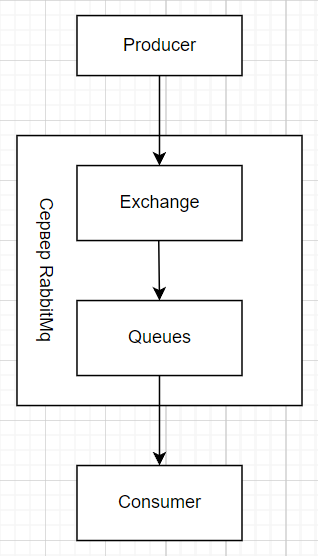
\includegraphics[width=0.7\textwidth]{rabbitMqArchitecture.png}
            \end{column}
        \end{columns}
    \end{frame}

    \begin{frame}
        \frametitle{Пример, Fanout Exchange}
        \begin{center}
            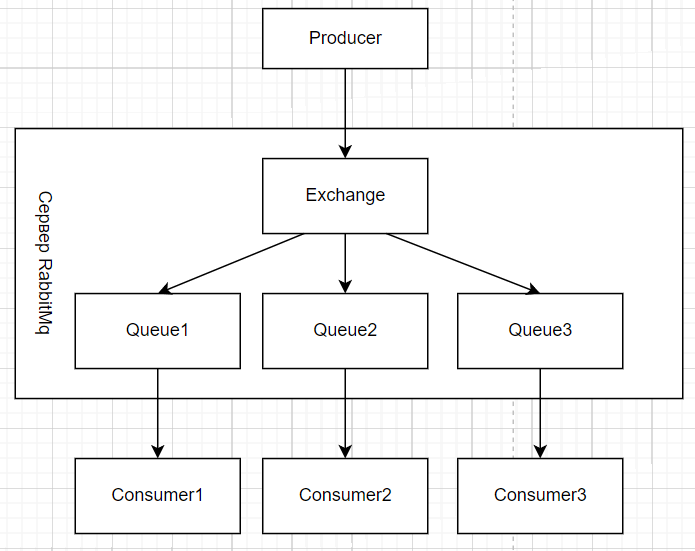
\includegraphics[width=0.5\textwidth]{fanoutExchange.png}
        \end{center}
    \end{frame}

    \begin{frame}
        \frametitle{Пример, Direct Exchange с темами}
        \begin{center}
            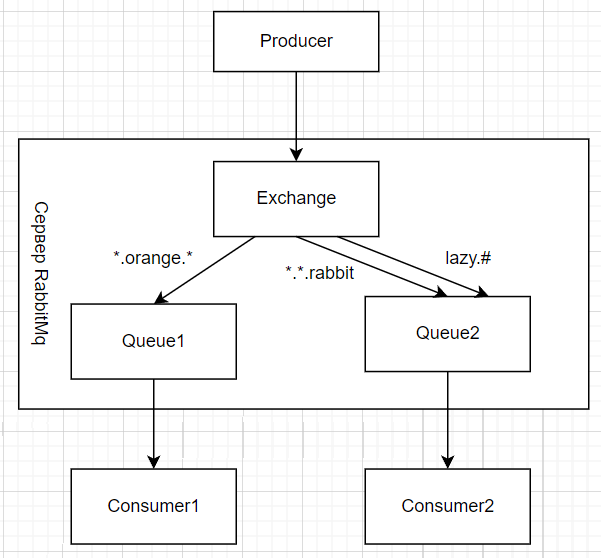
\includegraphics[width=0.5\textwidth]{topicExchange.png}
        \end{center}
        \begin{itemize}
            \item Routing key --- метаинформация для диспетчеризации сообщений (вида <<слово.слово.слово...>>)
        \end{itemize}
    \end{frame}

    \section{Пример}

    \begin{frame}[fragile]
        \frametitle{Пример, отправитель}
        \begin{ssmall}
            \begin{minted}{csharp}
using RabbitMQ.Client;
using System.Text;

var factory = new ConnectionFactory() { HostName = "localhost" };
using var connection = factory.CreateConnection();
using var channel = connection.CreateModel();

channel.QueueDeclare(queue: "hello",
    durable: false,
    exclusive: false,
    autoDelete: false,
    arguments: null);

var message = "Hello World!";
var body = Encoding.UTF8.GetBytes(message);

channel.BasicPublish(exchange: "",
    routingKey: "hello",
    basicProperties: null,
    body: body);

Console.WriteLine($" [x] Sent {message}");
            \end{minted}
        \end{ssmall}
    \end{frame}

    \begin{frame}[fragile]
        \frametitle{Пример, получатель}
        \begin{ssmall}
            \begin{minted}{csharp}
using RabbitMQ.Client;
using RabbitMQ.Client.Events;
using System.Text;

var factory = new ConnectionFactory() { HostName = "localhost" };
using var connection = factory.CreateConnection();
using var channel = connection.CreateModel();

channel.QueueDeclare(queue: "hello",
    durable: false,
    exclusive: false,
    autoDelete: false,
    arguments: null);

var consumer = new EventingBasicConsumer(channel);

consumer.Received += (model, ea) =>
{
    var body = ea.Body.ToArray();
    var message = Encoding.UTF8.GetString(body);
    Console.WriteLine($" [x] Received {message}");
};

channel.BasicConsume(queue: "hello",
    autoAck: true,
    consumer: consumer);
            \end{minted}
        \end{ssmall}
    \end{frame}

    \begin{frame}
        \frametitle{Как всё собрать и запустить}
        \begin{itemize}
            \item Поставить рантайм Erlang
            \item Поставить сервер RabbitMQ
            \begin{itemize}
                \item \url{https://www.rabbitmq.com/download.html}
            \end{itemize}
            \item Добавить зависимость от клиента RabbitMQ в проект
            \begin{itemize}
                \item .NET: RabbitMQ.Client в NuGet
                \item JVM: \mintinline{groovy}|compile group: 'com.rabbitmq', name: 'amqp-client', version: '5.14.2'|
            \end{itemize}
            \item Пролистать Getting Started 
            \begin{itemize}
                \item \url{https://www.rabbitmq.com/getstarted.html}, часть 1
            \end{itemize}
        \end{itemize}
    \end{frame}

    \section{Задача}

    \begin{frame}
        \frametitle{Задача на пару}
        В командах по два-три человека реализовать консольный сетевой чат на RabbitMQ
        \begin{itemize}
            \item Сервер для обмена сообщениями, о котором договариваются клиенты
            \begin{itemize}
                \item Центральный сервер, задаваемый как параметр командной строки (127.0.0.1 по умолчанию)
            \end{itemize}
            \item Есть именованные каналы, на которые можно переключаться и постить туда
            \begin{itemize}
                \item Должна быть команда подписки на канал, типа <<!switch channel1>>
                \item Начальный канал принимается как аргумент командной строки
                \item Переключение на несуществующий канал должно его создавать
            \end{itemize}
            \item Нет истории, получать только те сообщения, что были опубликованы с момента подключения
            \begin{itemize}
                \item Может помочь \url{https://www.rabbitmq.com/tutorials/tutorial-three-dotnet.html}
            \end{itemize}
        \end{itemize}
    \end{frame}

\end{document}